% N15, after eq:decision-two-arm-information-value and the 1.2 comparison.
图~\ref{fig:decision-two-round-exploration}把这两条选择路径展开。第一轮的平均收益相同，
但未知臂的结果改变参数后验，从而改变第二轮的最优行动。
\begin{figure*}[htbp]
  \centering
  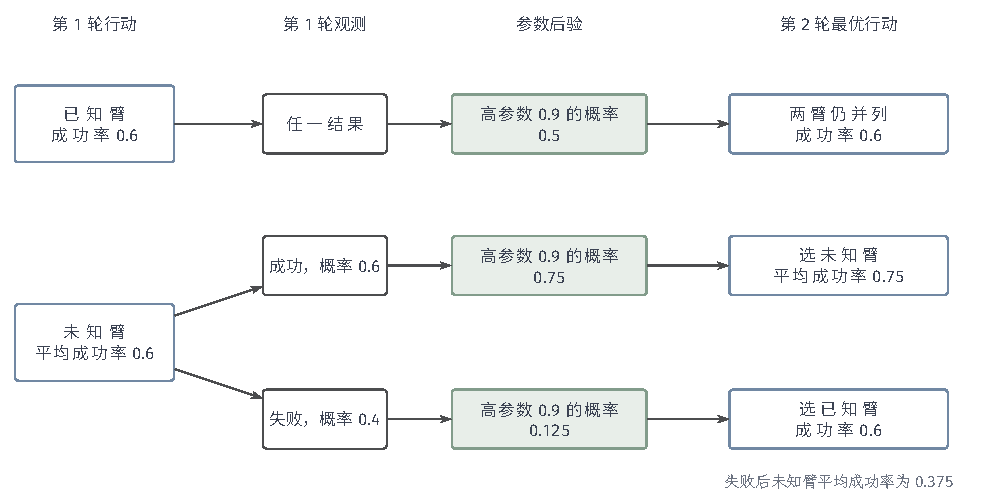
\includegraphics[width=169mm]{figures/02-mathematical-preliminaries-lower/02-dynamical-systems-control-decision-and-games/tikz/decision-two-round-exploration/figure.pdf}
  \caption{两轮选择中的探索价值。参数\(\Theta\in\{0.3,0.9\}\)在两轮间不变，先验各为\(1/2\)；
  给定参数，各次奖励条件独立，每轮只观察所选臂。后验列给出高参数的概率，末列给出下一轮最优行动的成功率。
  先选未知臂的两轮期望为\(0.6+0.6\times0.75+0.4\times0.6=1.29\)，先选已知臂为\(1.2\)。}
  \label{fig:decision-two-round-exploration}
\end{figure*}

% N16, after I2 definition and explanation, before the existing table.
图~\ref{fig:game-card-history-information}保留两条真实质询历史，并以同一信息集连接参与者2的决策节点。
两处行动概率相同来自信息约束，不能随隐藏牌面分别设定。
\begin{figure*}[htbp]
  \centering
  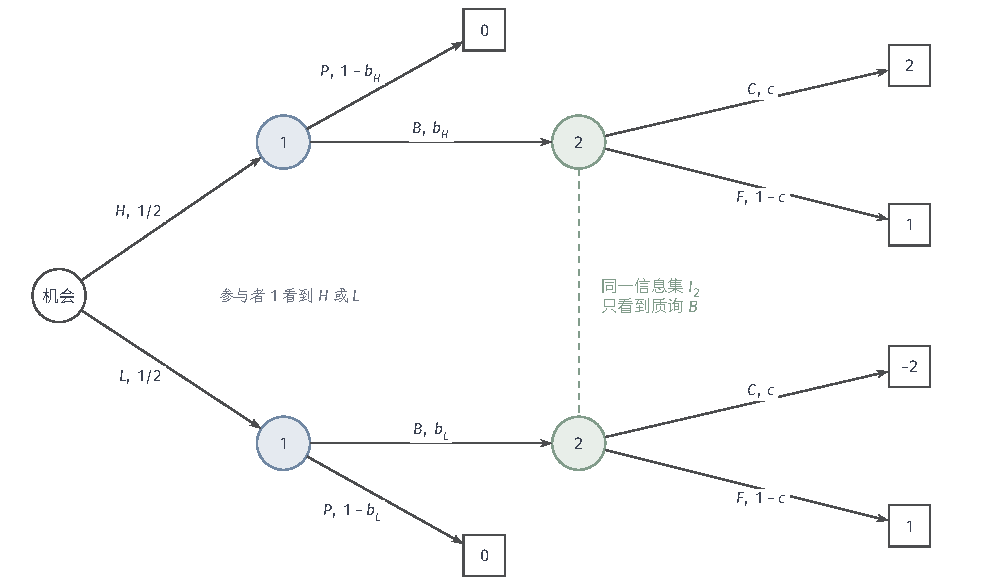
\includegraphics[width=169mm]{figures/02-mathematical-preliminaries-lower/02-dynamical-systems-control-decision-and-games/tikz/game-card-history-information/figure.pdf}
  \caption{三张牌教学博弈的历史树。机会仅在高牌\(H\)与低牌\(L\)间等概率发牌，公共中牌\(M\)是比较基准。
  参与者1看到牌面，分别以\(b_H,b_L\)质询；参与者2只看到质询，虚线连接的信息集\(I_2\)中共用应对概率\(c\)。
  方节点标出终局收益\(u_1\)，参与者2的收益为\(-u_1\)。虚线表示无法区分的历史，不是额外行动或转移。}
  \label{fig:game-card-history-information}
\end{figure*}
